\chapter*{Appendices}
\addcontentsline{toc}{chapter}{Appendices}

\appendix

\chapter{How to connect to SALSA using Nomachine 4}
\label{app:nomachine}
The program NoMachine 4 can be used to connect to the control computers brage or vale.
This tutorial was compiled using the program Nomachine 4.0.366 for Windows XP/7/8 available
from http://www.nomachine.com 2013-11-25. It might also be useful for connecting with 
NoMachine 4.0 on Mac (OS X) or Unix/Linux although the tutorial has not been tested on these systems.

\section{Quick summary}
When creating your connection you need to use Protocol: SSH, and also press the
button "Advanced" on the same screen and choose number two: "Use the NoMachine
login" to authenticate on host. See figures \ref{fig:create} and
\ref{fig:advanced}. 

\section{Connecting: Step-by-step instructions}
In this example we will be connecting to a SALSA control computer called
\emph{vale} using the program Nomachine 4.0.366 for Windows XP/7/8 available at
www.nomachine.com. First, download and Install the Nomachine program. Then,
start the NoMachine program (e.g. using the shortcut on your desktop) and click
continue through the welcome screens until you arrive at the screen
\emph{Recent connections} shown in fig. \ref{fig:recentconn}. From here, follow
the instructions in the figure captions.

\begin{figure}[H]
    \centering
    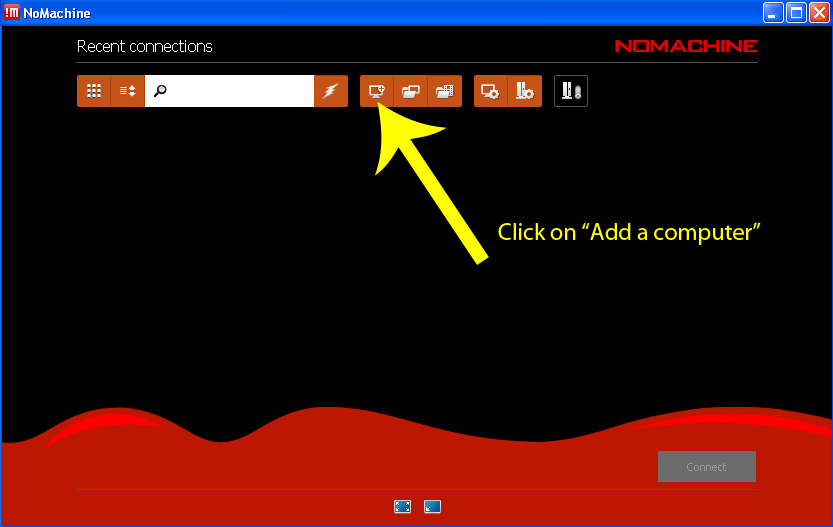
\includegraphics[height=0.25\paperheight]{../figures/nomachinefigs/fig1_recentconn.png}
    \caption{The startup screen of Nomachine 4 after clicking through the welcome instructions. Click on \emph{Add computer} marked with an arrow here.}
    \label{fig:recentconn}
\end{figure}

\begin{figure}[H]
    \centering
    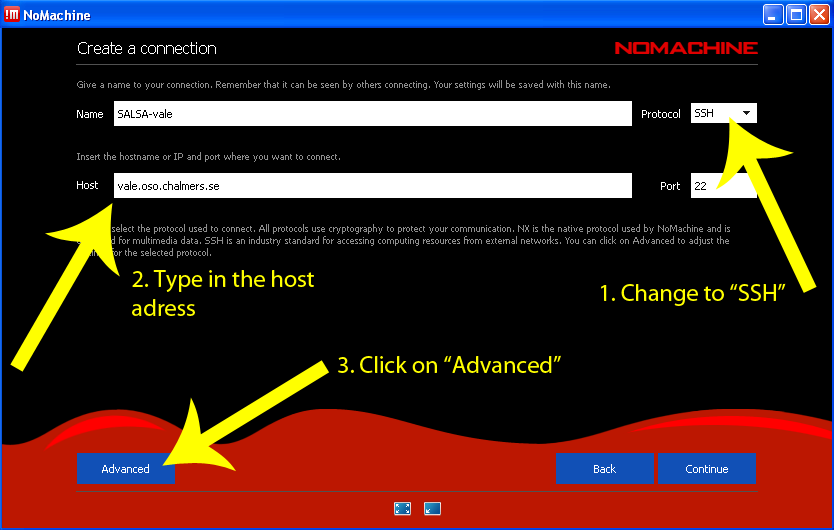
\includegraphics[height=0.25\paperheight]{../figures/nomachinefigs/fig2_create.png}
    \caption{The screen for creating a new connection. Here you need to change the host adress, the protocol to SSH and finally click on the button \emph{Advanced}.}
    \label{fig:create}
\end{figure}

\begin{figure}[H]
    \centering
    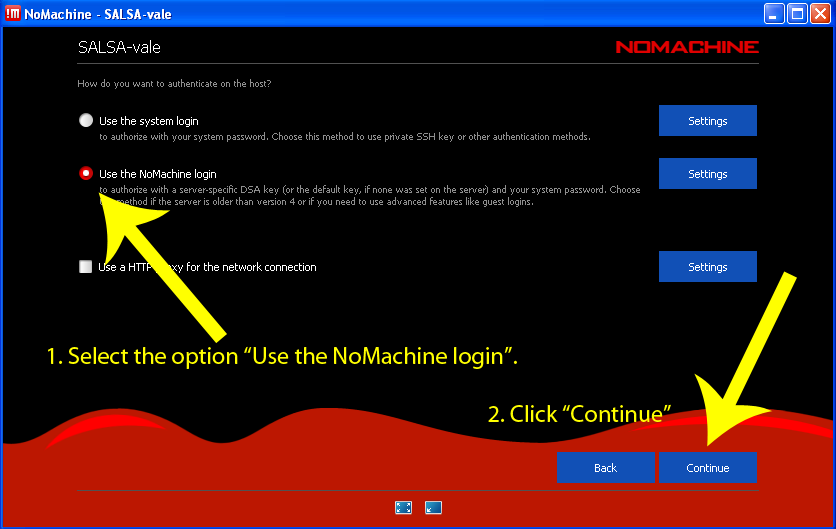
\includegraphics[height=0.25\paperheight]{../figures/nomachinefigs/fig3_advanced.png}
    \caption{After you click \emph{Advanced} you need to select option 2: "Use the NoMachine login", see fig. \ref{fig:advanced}. Then press \emph{Continue}.}
    \label{fig:advanced}
\end{figure}

\begin{figure}[H]
    \centering
    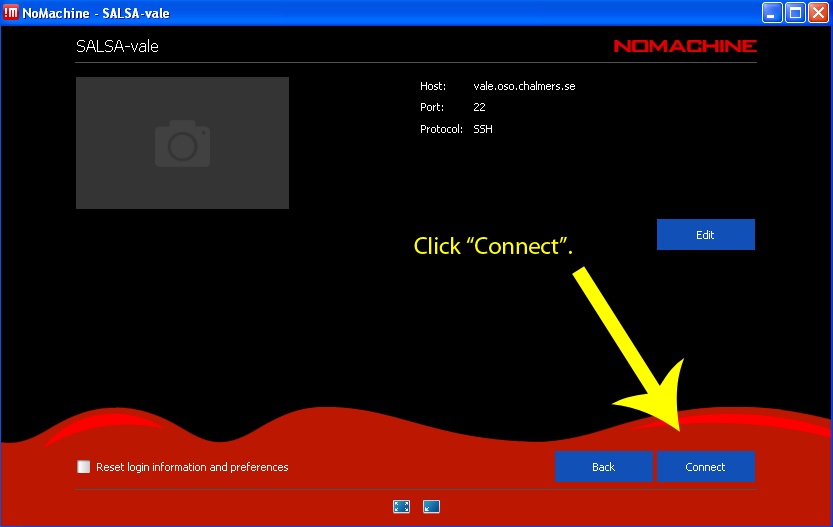
\includegraphics[height=0.25\paperheight]{../figures/nomachinefigs/fig4_connect.png}
    \caption{Verify that the host adress is correct, e.g. vale.oso.chalmers.se to connect to the computer "vale" or brage.oso.chalmers.se to connect to "brage", and that "Port:22" and "Protocol:SSH", then click \emph{Connect}.}
    \label{fig:connect}
\end{figure}

\begin{figure}[H]
    \centering
    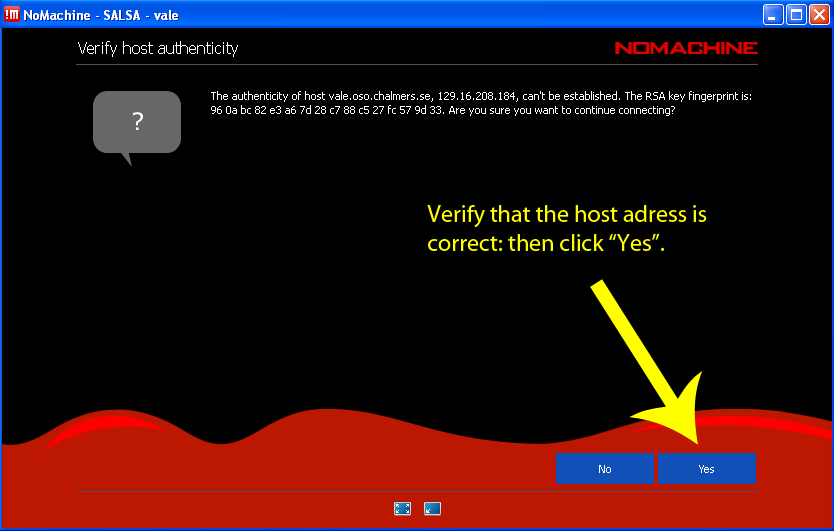
\includegraphics[height=0.25\paperheight]{../figures/nomachinefigs/fig5_verify.png}
    \caption{The first time you connect you will get a warning to "Verify host authenticity". Check that the host adress is indeed correct, then click \emph{Yes}.}
    \label{fig:verify}
\end{figure}

\begin{figure}[H]
    \centering
    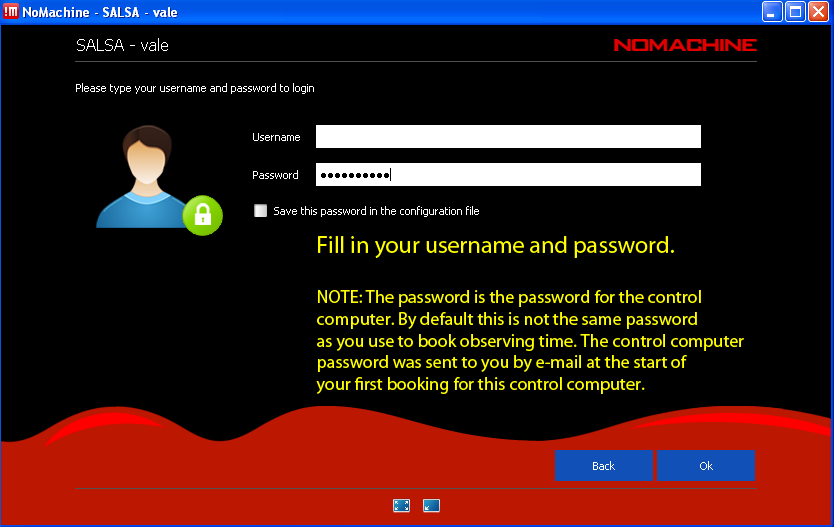
\includegraphics[height=0.25\paperheight]{../figures/nomachinefigs/fig6_userpass.png}
    \caption{Fill in your username and password. Then click \emph{OK}. 
{\bf Note:} Here you need to use your ``telescope password'', which may be different
than the password you use to book observing time. Check the SALSA-webpage, under ``My account'' to find your telescope password.}
    \label{fig:userpass}
\end{figure}

\begin{figure}[H]
    \centering
    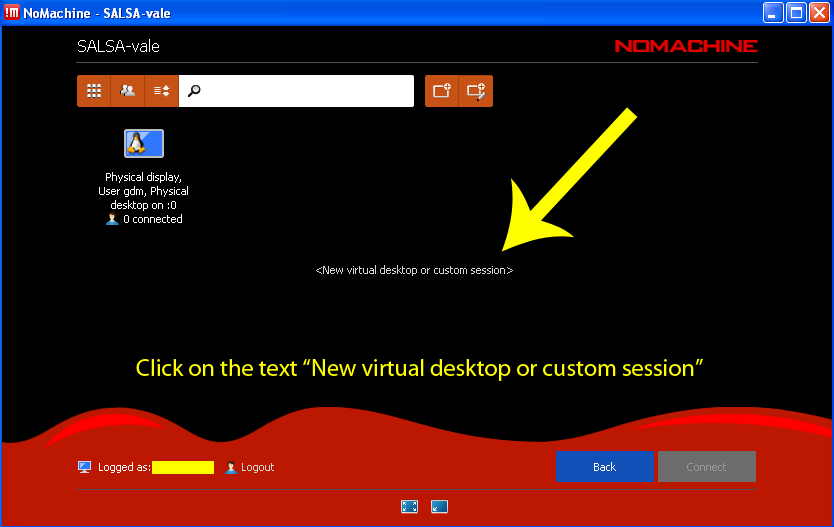
\includegraphics[height=0.25\paperheight]{../figures/nomachinefigs/fig7_session.png}
    \caption{Click on the text in the middle of the screen \emph{New virtual desktop or custom session}. }
    \label{fig:session}
\end{figure}

\begin{figure}[H]
    \centering
    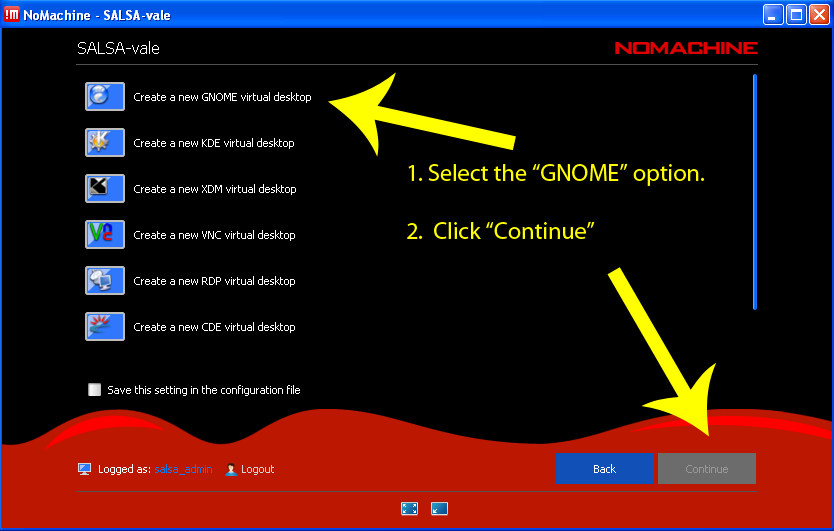
\includegraphics[height=0.25\paperheight]{../figures/nomachinefigs/fig8_gnome.png}
    \caption{Select the "Gnome" option in the list and then click \emph{Continue}. You may now
see a few info screens from NoMachine on which you may only click OK.}
    \label{fig:gnome}
\end{figure}

\begin{figure}[H]
    \centering
	
\includegraphics[width=0.9\textwidth]{../figures/nomachinefigs/fig9-connected.pdf}
    \caption{Hopefully you will (perhaps after a few NoMachine info screens)
see something like this. Congratulations - You are now connected to the SALSA
control computer and you may start observing! 
To start using the telescope, double-click on the shortcut to "SALSA".} \label{fig:connected}
\end{figure}

